\begin{minipage}[t]{180mm}
\fcolorbox{black}{white}{
\begin{minipage}[b]{30mm}

\includegraphics[width=0.5\linewidth]{unflogo.pdf}
\end{minipage}
\begin{minipage}[b]{100mm}
\Huge \textbf{UNF NEWZ} \\
\Large -- Søvn og retsstavning er overvurderet! 
\end{minipage}
\begin{minipage}[b]{50mm}
\Large Onsdag 17.07.2015 \\
\normalsize Redigeret i \LaTeX\ af \\ SOM, MGS, MMN, SABH
\end{minipage}
}
\end{minipage}



\begin{minipage}[b]{0.95\linewidth}
\begin{minipage}[t]{0.47\textwidth}
\vspace{3mm}

\section*{Velkomst}
Kære deltagere,

I har nu begivet jer på en rejse mod solopgangen, i håbet om at finde frelsen i matematik. Frygt ikke, I er kommet det rette sted, fra her er der kun to veje, lysets og mørkets. Lysets vej er nemmest, men anvendt frem for dyb, det er fysikerens og datalogens forfejlede retning, fyldt med usikkerheder og manglende forståelse for den ægte sandhed. Her er vi på vejen mod mørket, omgivet af mangfoldigheder og indlejret i rum, hvis indre produkt sandeligt er positiv og definit.

Det var i herrens år 2007, da barbariet endte og mennesket blev sig selv bevidst. En mørk sommeraften mødtes forskrækkede matematikere ved Odins vig for at aksiomatisere livet og verden. Sidenhen, hver gang året står på sit højeste, mødes de, sidenhen skiftende steder på den jydske hede og på mons Hafniae.

Svensken truer mod øst, og Jyden truer mod vest, men dette skal ikke bekymre jer endnu, angsten kan vente til mandag. Fryd jer, mød hinanden, lær og læs og dø kun når I har fået lov. 

{\flushright\emph{Jeres co-koordinator, Helene}}

\section*{Velkomst}
Kære deltagere,

I har nu begivet jer på en rejse mod solopgangen, i håbet om at finde frelsen i matematik. Frygt ikke, I er kommet det rette sted, fra her er der kun to veje, lysets og mørkets. Lysets vej er nemmest, men anvendt frem for dyb, det er fysikerens og datalogens forfejlede retning, fyldt med usikkerheder og manglende forståelse for den ægte sandhed. Her er vi på vejen mod mørket, omgivet af mangfoldigheder og indlejret i rum, hvis indre produkt sandeligt er positiv og definit.

Det var i herrens år 2007, da barbariet endte og mennesket blev sig selv bevidst. En mørk sommeraften mødtes forskrækkede matematikere ved Odins vig for at aksiomatisere livet og verden. Sidenhen, hver gang året står på sit højeste, mødes de, sidenhen skiftende steder på den jydske hede og på mons Hafniae.

Svensken truer mod øst, og Jyden truer mod vest, men dette skal ikke bekymre jer endnu, angsten kan vente til mandag. Fryd jer, mød hinanden, lær og læs og dø kun når I har fået lov. 

{\flushright\emph{Jeres co-koordinator, Morten Agger}}

\end{minipage}
\hfill\begin{minipage}[t]{0.47\textwidth}

\vspace{1mm}
\tikzstyle{mybox} = [draw=white, fill=blue!20, very thick,
    rectangle, rounded corners, inner sep=10pt, inner ysep=20pt]
\tikzstyle{fancytitle} =[fill=red, text=white]

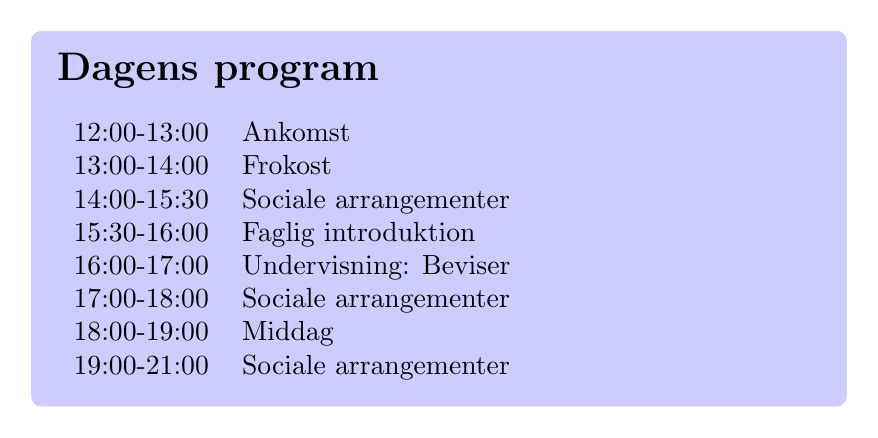
\begin{tikzpicture}
\node [mybox] (box){%
\begin{minipage}{0.80\textwidth}
\vspace{-4mm}\section*{Dagens program}
\begin{tabular}{ll}
12:00-13:00 & Ankomst \\
13:00-14:00 & Frokost \\
14:00-15:30 & Sociale arrangementer \\
15:30-16:00 & Faglig introduktion \\
16:00-17:00 & Undervisning: Beviser \\
17:00-18:00 & Sociale arrangementer \\
18:00-19:00 & Middag \\
19:00-21:00 & Sociale arrangementer \\
\end{tabular}
\vspace{-4mm}
\end{minipage}
};
\end{tikzpicture}%

\section*{Velkommen til Matematik Camp!}
Kære deltagere!\\
Det er mig en udsøgt glæde at velkomme jer alle sammen til en uge under min kompetente ledelse! I denne uge vil i udvikle jer til bedre og mere disciplinerede mennesker, der ikke bare bliver bedre matematikere og lære at gå frem med nye Metriker, i vil lære god takt og tone og hvordan rigtige mennesker opføre sig. For at opfylde dette ekstra mål har jeg i år valgt at tilføje et par simple regler som i, som deltager, skal overholde. For det første vil det på årets Matematik Camp ikke være tillad at stå eller side i rundkreds, da dette er utrolig uhøfligt over for firkanter. Af andre simple regler kan nævnes at, når man starter med at gå skal man altid starte med venstre ben, farven blå er bandlyst, længere varende øjenkontakt er strengt forbudt og folk der går stik øst vil blive bordvist. Målet med disse rimelige regler er at assimilere alle jer uslebne små pjok ind til en hærdet hær af uge matematikere. Deltagere som ikke kan overholde disse simple og let følgelige regler vil blive sat til at skrive haiku digte til de dør af sult. Til slut vil jeg gerne endnu en gang byder jer alle sammen velkommen, ydredørene er allerede låst og vil først blive låst op lørdag eftermiddag, og jeg vil dedikere hver en time jeg har ind til da på at få jer formet som sande matematikere.

 
{\flushright\emph{Jeres koordinator, Morten Grue Sørensen}}

\begin{center}
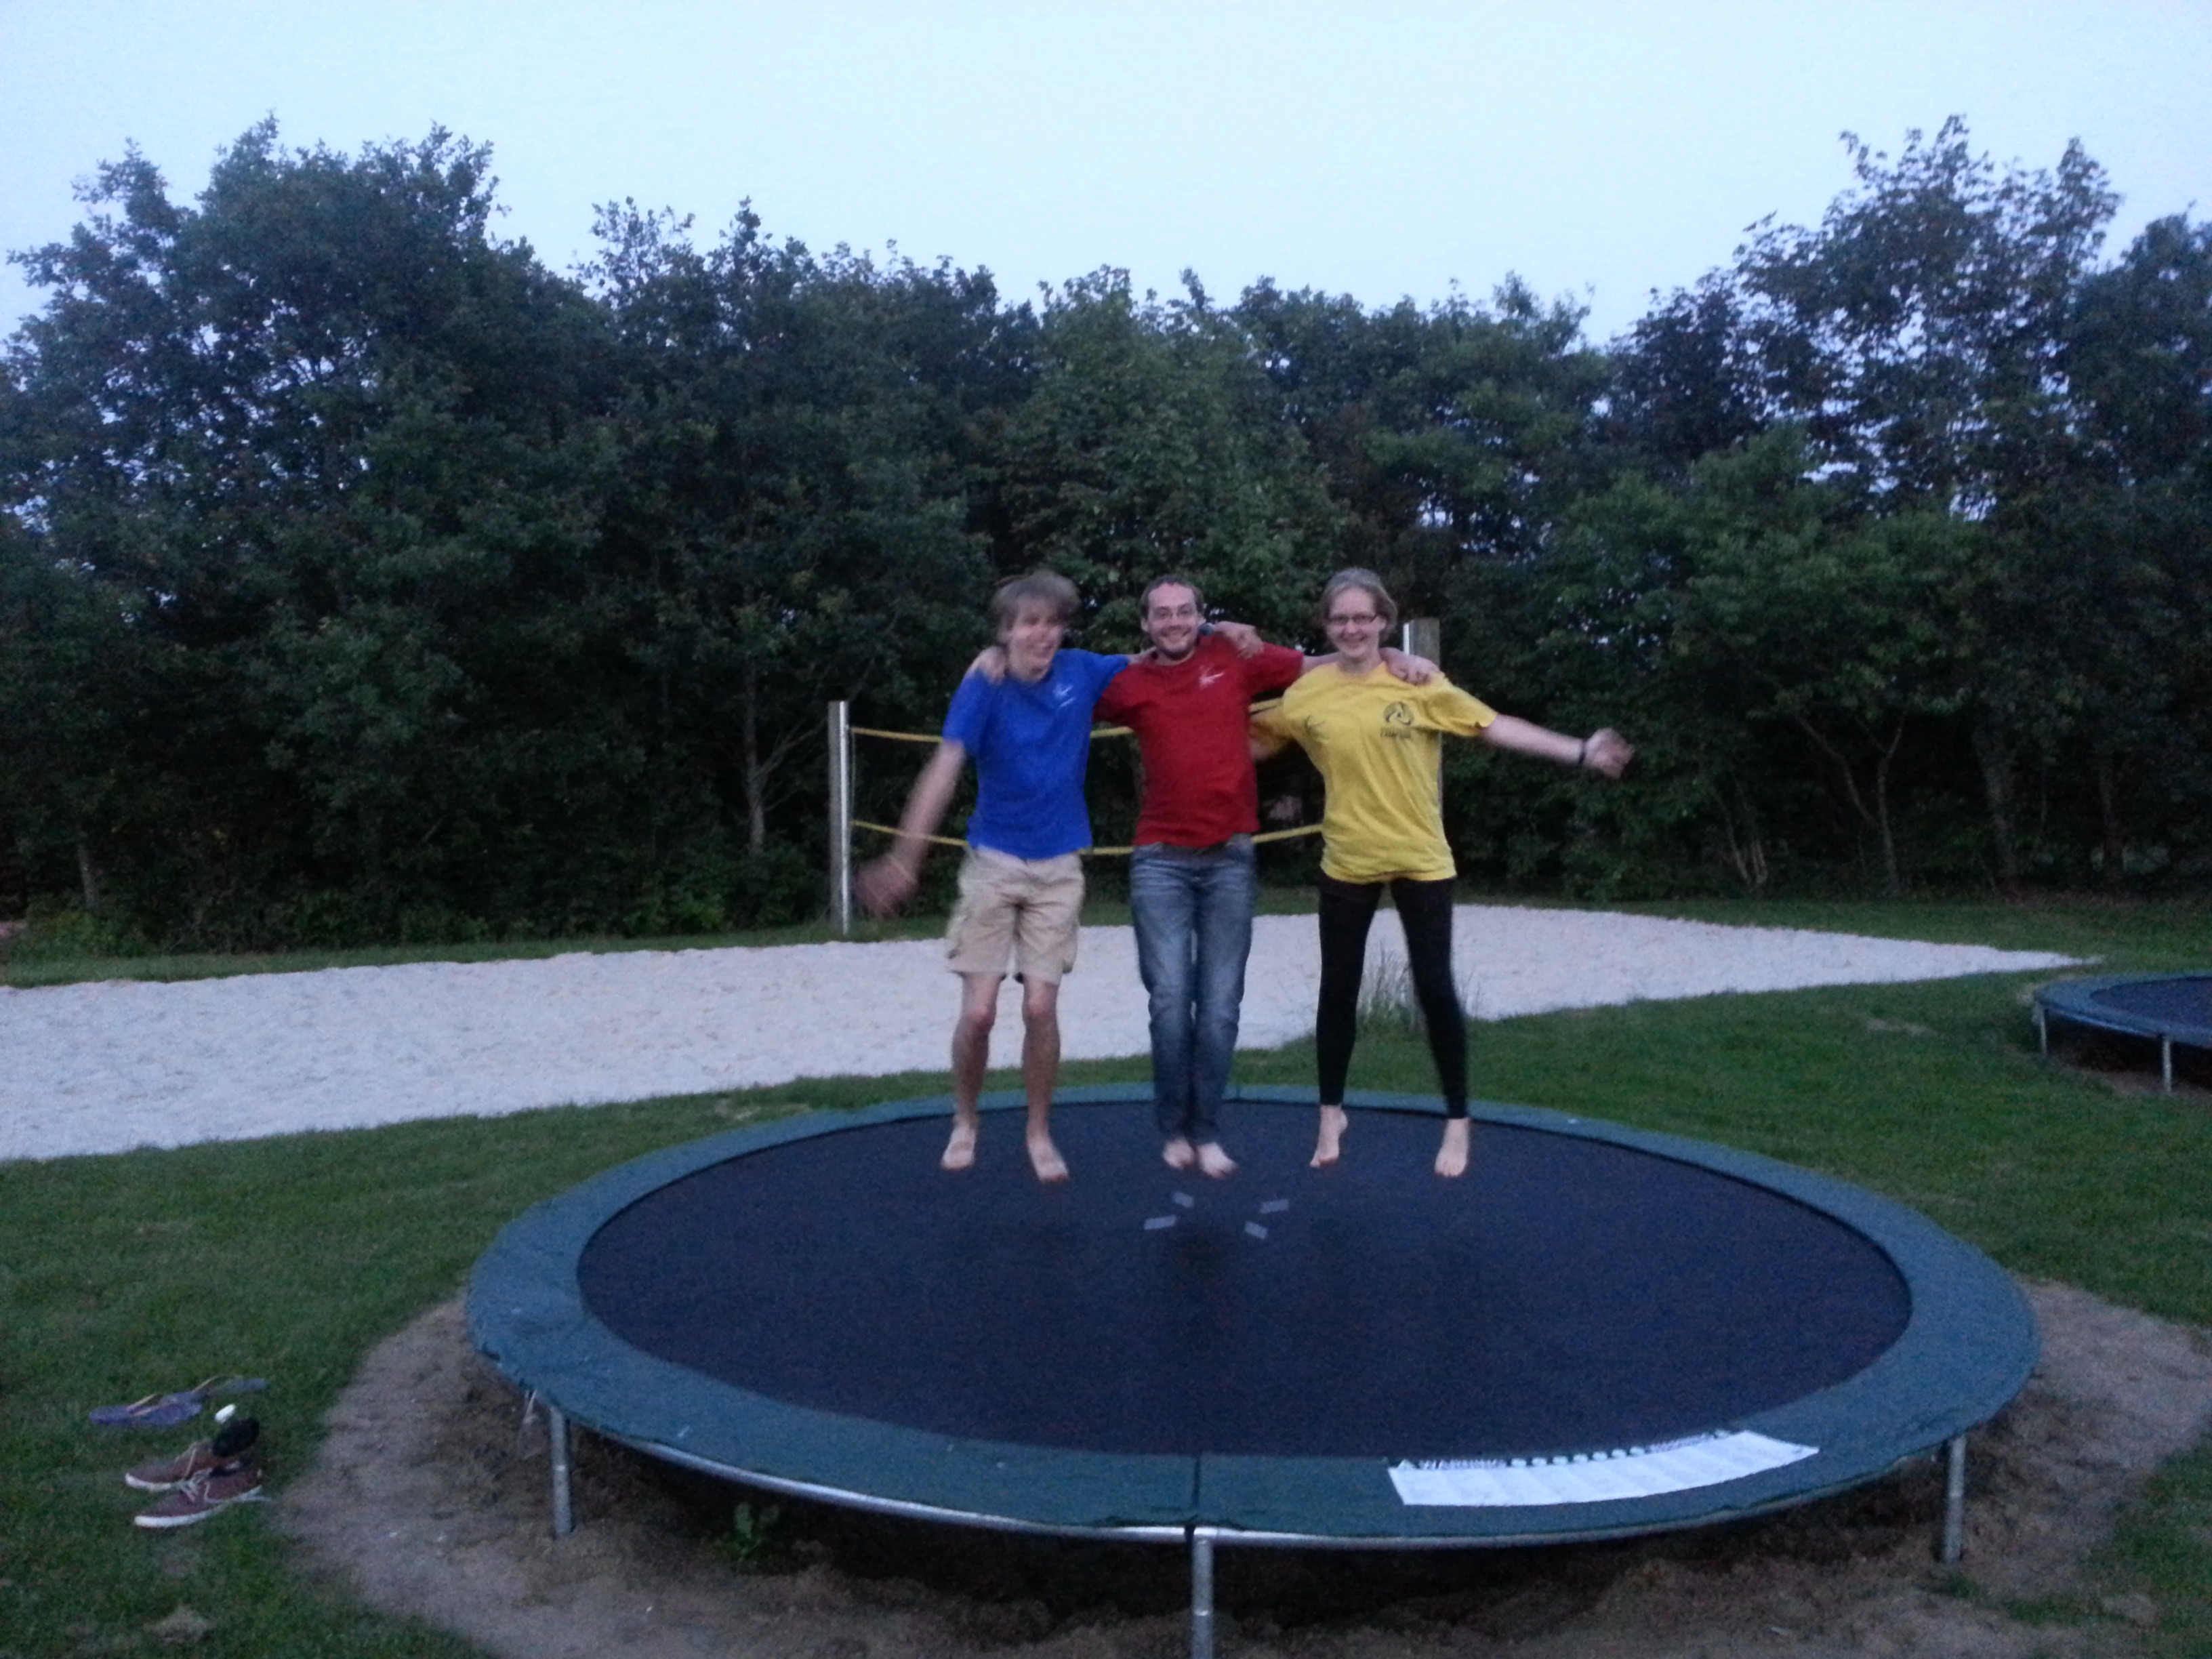
\includegraphics[width=\linewidth]{koordinatorer.jpg}
\end{center}

\end{minipage}
\end{minipage}
